\subsection{实验目的}
理解监督分类的概念,掌握一些典型的监督分类方法,例如线性判别法。完成遥感图像的图像分类。
\subsection{实验原理}
\begin{description}
	\item[监督分类的概念] 首先使用训练样本学习一个分类器,再对测试样本进行分类。
	\item[图像分类的两个步骤] 特征提取与分类算法。
	\item[特征提取] 颜色特征向量。
	\item[分类-训练过程] 使用训练样本学习分类器。
	\item[分类-测试过程] 使用学习好的分类器对测试样本分类。
\end{description}
\subsubsection{线性判别函数的定义}
直接用来对模式进行分类的准则函数。

若分属于$\omega_1$,$\omega_2$的两类模式可用一方程$d(\mathbf{X})=0$来划分,那么称$d(\mathbf{X})$为判别函数,或称判决函数、决策函数。
\begin{figure}[H]
	\centering
	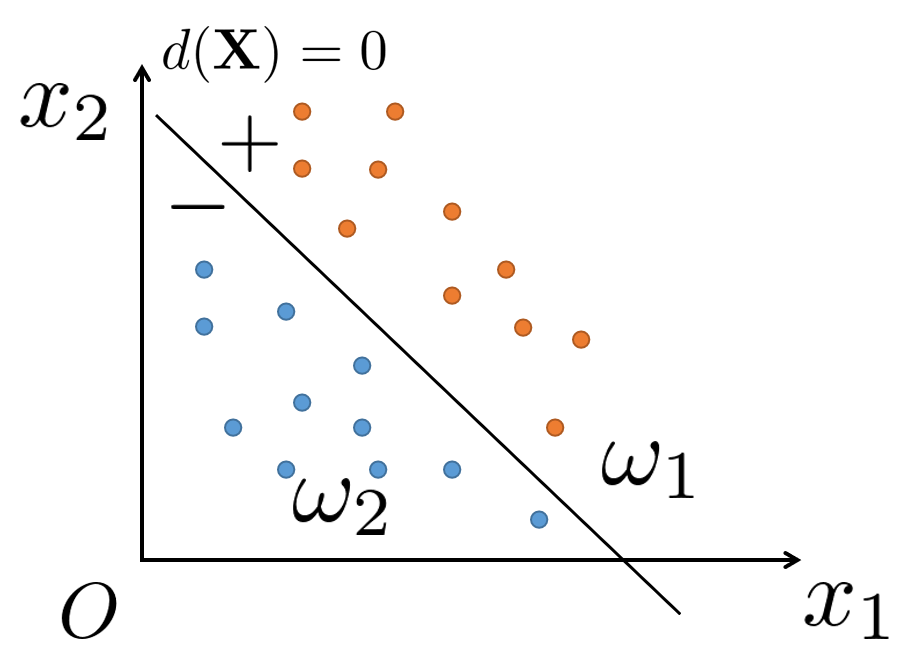
\includegraphics[width=0.7\linewidth]{figure/exp5classification}
	\caption{二类二维样本的分布}
	\label{fig:exp5classification}
\end{figure}
\begin{quote}
	\kaishu 例:一个二维的两类判别问题,模式分布如图所示,这些分属于$\omega_1$,$\omega_2$两类的模式可用一直线方程$d(\mathbf{X})=0$来划分。
	\[ d(\mathbf{X})=w_1x_1+w_2x_2+w_3=0 \]
	式中:$x_1$,$x_2$为坐标变量,$w_1$,$w_2$,$w_3$为方程参数。
\end{quote}
\subsubsection{多类情况}
\begin{description}
	\item[$\omega_i/\bar{\omega_i}$两分法] 用线性判别函数将属于$\omega_i$类的模式与其余不属于$\omega_i$类的模式分开。
\end{description}
\[ d_i(\mathbf{X})=\mathbf{W}_i^\mathsf{T}\mathbf{X}\begin{cases}
>0,\quad& \mathbf{X}\in\omega_i \\
<0,\quad& \mathbf{X}\in\bar{\omega_i}
\end{cases} \quad i=1,2,\dots,M \]
识别分类时:将某个待分类模式$\mathbf{X}$分别带入$M$个类的$d(\mathbf{X})$中,若只有$d(\mathbf{X})>0$,其他$d(\mathbf{X})$均$<0$,则判为$\omega_1$类。

对样本进行规范化处理,即$\omega_2$类样本全部乘以$(-1)$,则有
\[ d(\mathbf{X})=\mathbf{W}^\mathsf{T}\mathbf{X}>0 \]
感知器算法通过对已知类别的训练样本集的学习,寻找一个满足上式的权向量。

感知机算法步骤:
\begin{enumerate}
	\item 选择$N$个分属于$\omega_1$和$\omega_2$类的模式样本构成训练样本集
	\[ \left\lbrace \mathbf{X}_1,\mathbf{X}_2,\dots,\mathbf{X}_N \right\rbrace \]
	构成增广向量形式,并进行规范化处理。任取权向量初始值$\mathbf{W}(1)$,开始迭代,迭代次数$k=1$。
	\item 用全部训练样本进行一轮迭代,计算$\mathbf{W}^\mathsf{T}(k)\mathbf{X}_i$的值,并修正权向量。分两种情况更新权向量的值:
	\begin{enumerate}
		\item 若$\mathbf{W}^\mathsf{T}(k)\mathbf{X}_i\leq 0$,分类器对第$i$个模式做了错误的分类。权向量矫正为:$\mathbf{W}(k+1)=\mathbf{W}(k)+c\mathbf{X}_i$($c$:正的矫正增量)。
		\item 若$\mathbf{W}^\mathsf{T}(k)\mathbf{X}_i> 0$,分类正确,权向量不变
		\[ \mathbf{W}(k+1)=\mathbf{W}(k) \]
	\end{enumerate}
	统一写为
	\[ \mathbf{W}(k+1)=\begin{cases}
	\mathbf{W}(k),\quad & \text{若}\mathbf{W}^\mathsf{T}(k)\mathbf{X}_i > 0 \\
	\mathbf{W}(k)+c\mathbf{X}_i, \quad & \text{若}\mathbf{W}^\mathsf{T}(k)\mathbf{X}_i \leq 0
	\end{cases} \]
	\item 分析分类结果:只要有一个错误分类,回到$2$,直至对所有样本正确分类。
\end{enumerate}
\subsection{实验流程}
\begin{figure}[H]
	\centering
	\begin{tikzpicture}[node distance=1.5cm]
	\node (start)[startstop] {开始};
	\node (inputimg)[io, below of=start] {输入待分类的图片};
	\node (select_training_set)[process, below of=inputimg] {选取训练样本集};
	\node (generate_negative_training_set)[process, below of=select_training_set] {生成负训练样本集};
	\node (initialize_weight)[process, below of=generate_negative_training_set] {初始化权重矩阵};
	\node (optimize_weight)[process, below of=initialize_weight] {迭代优化权重矩阵};
	\node (classifing_image)[process, below of=optimize_weight] {对全图进行分类};
	\node (ouput_classification)[io, below of=classifing_image] {输出分类结果};
	\node (end)[startstop, below of=ouput_classification] {结束};
	
	\draw[arrow] (start) -- (inputimg);
	\draw[arrow] (inputimg) -- (select_training_set);
	\draw[arrow] (select_training_set) -- (generate_negative_training_set);
	\draw[arrow] (generate_negative_training_set) -- (initialize_weight);
	\draw[arrow] (initialize_weight) -- (optimize_weight);
	\draw[arrow] (optimize_weight) -- (classifing_image);
	\draw[arrow] (classifing_image) -- (ouput_classification);
	\draw[arrow] (ouput_classification) -- (end);
	\end{tikzpicture}
	\caption{监督分类流程图}
\end{figure}
\subsection{实验程序}
\lstinputlisting[caption={LDA监督分类程序}]{"../Executable Script/Exp 5/ReadViaductImage.m"}
\subsection{实验结果和分析}
对如图\ref{fig:viaduct_52}所示的图片进行分类
\begin{figure}[H]
	\centering
	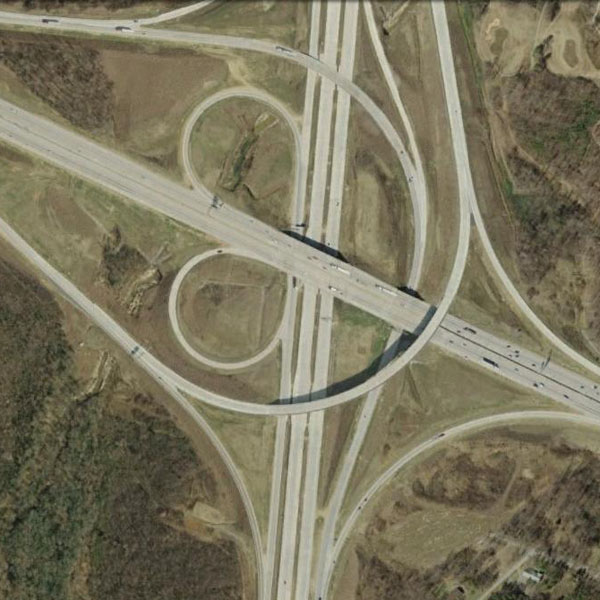
\includegraphics[width=0.7\linewidth]{figure/viaduct_52.jpg}
	\caption{待分类原图像}
	\label{fig:viaduct_52}
\end{figure}
首先选择用于训练权重矩阵的训练样本,训练样本的位置如图\ref{fig:viaduct_52_training_set}所示
\begin{figure}[H]
	\centering
	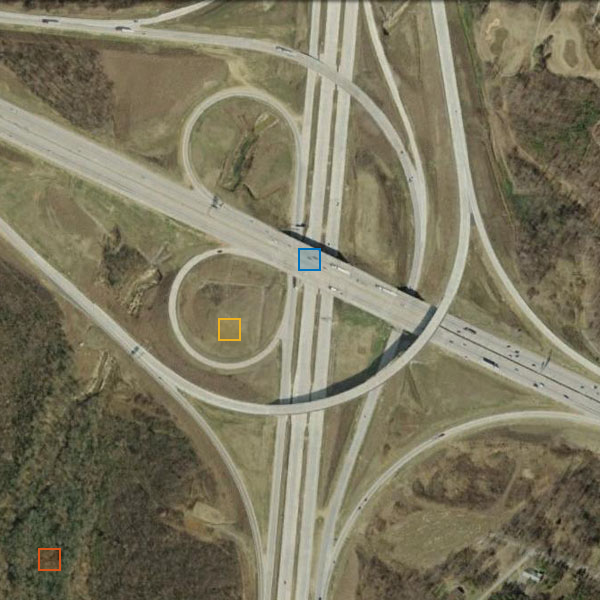
\includegraphics[width=0.7\linewidth]{figure/viaduct_52_Training_Set_Marker.png}
	\caption{标记训练样本的位置}
	\label{fig:viaduct_52_training_set}
\end{figure}
图中,标记为蓝色区域的是道路样本,标记为红色区域的是植被样本,标记为黄色区域的是土地样本。选择标记好的样本生成正向样本集和负向样本集,使用这些样本对权重矩阵的12个参数进行训练。

训练完成后,可以对全图进行分类,分类结果如图\ref{fig:viaduct_52_road_logic}、图\ref{fig:viaduct_52_grass_logic}和图\ref{fig:viaduct_52_ground_logic}所示。
\begin{figure}[H]
	\centering
	\begin{minipage}{0.3\linewidth}
		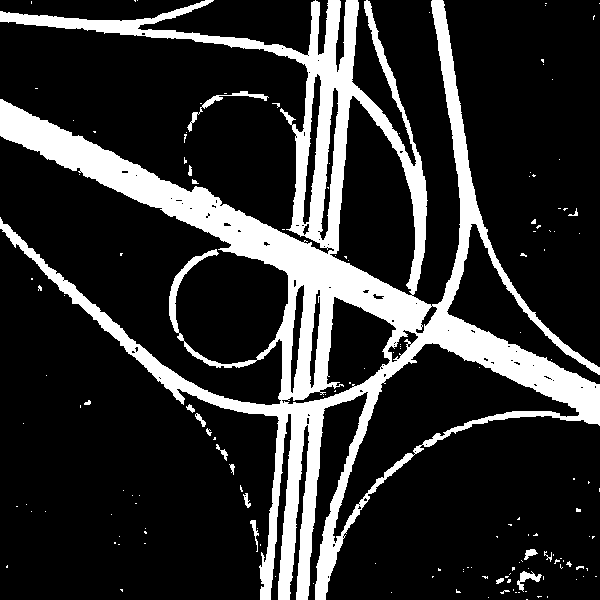
\includegraphics[width=\linewidth]{figure/viaduct_52_Road_Logic_P.png}
		\caption{道路分类结果}
		\label{fig:viaduct_52_road_logic}
	\end{minipage}
	\begin{minipage}{0.3\linewidth}
		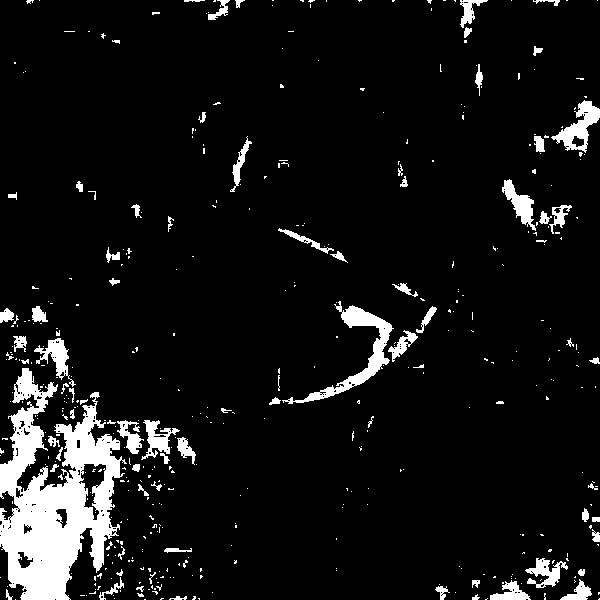
\includegraphics[width=\linewidth]{figure/viaduct_52_Grass_Logic_P.png}
		\caption{植被分类结果}
		\label{fig:viaduct_52_grass_logic}
	\end{minipage}
	\begin{minipage}{0.3\linewidth}
		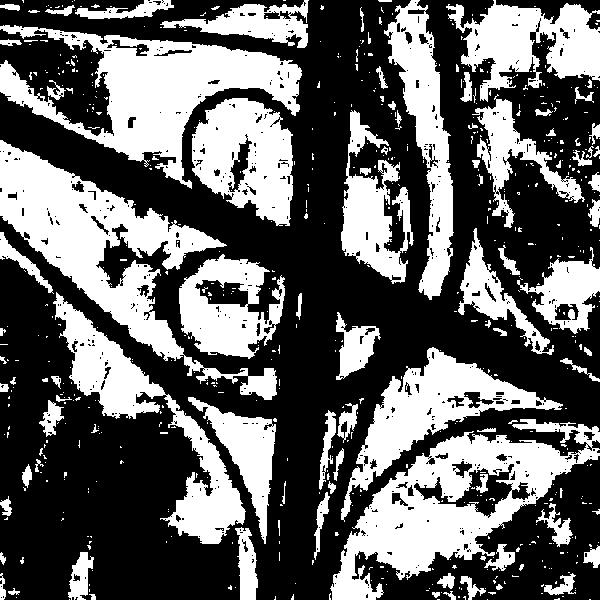
\includegraphics[width=\linewidth]{figure/viaduct_52_Ground_Logic_P.png}
		\caption{土地分类结果}
		\label{fig:viaduct_52_ground_logic}
	\end{minipage}
\end{figure}
对原图片中的不同分类进行分离,可以得到如图\ref{fig:viaduct_52_road_separated}、图\ref{fig:viaduct_52_grass_separated}和图\ref{fig:viaduct_52_ground_separated}所示的结果
\begin{figure}[H]
	\centering
	\begin{minipage}{0.3\linewidth}
		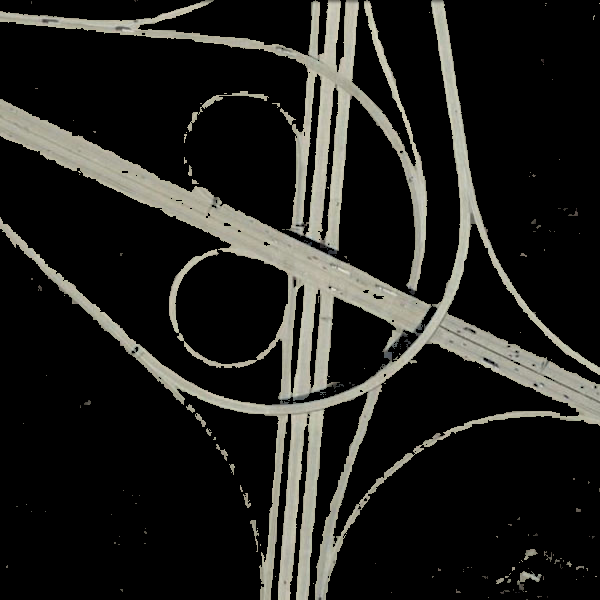
\includegraphics[width=\linewidth]{figure/viaduct_52_Road_Separated_P.png}
		\caption{道路分类结果}
		\label{fig:viaduct_52_road_separated}
	\end{minipage}
	\begin{minipage}{0.3\linewidth}
		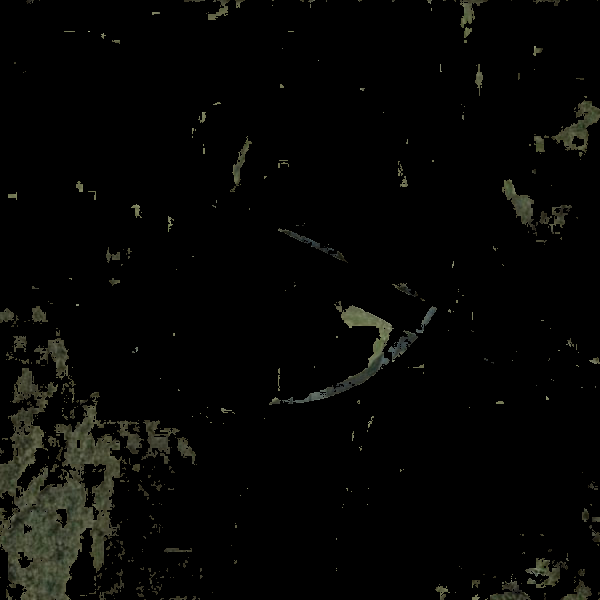
\includegraphics[width=\linewidth]{figure/viaduct_52_Grass_Separated_P.png}
		\caption{植被分类结果}
		\label{fig:viaduct_52_grass_separated}
	\end{minipage}
	\begin{minipage}{0.3\linewidth}
		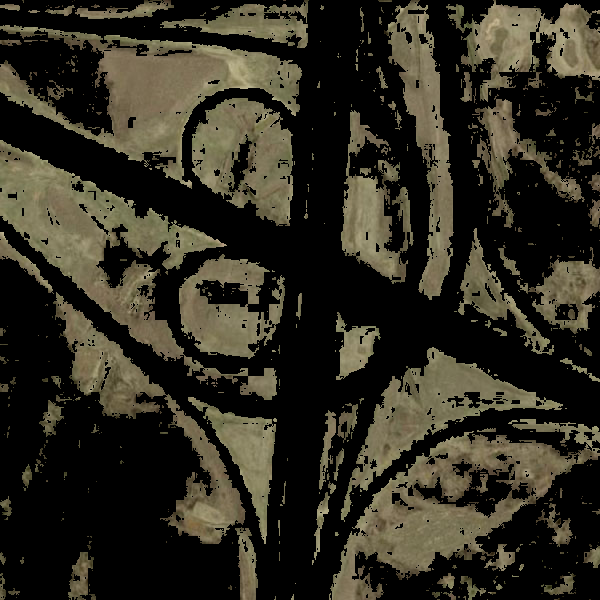
\includegraphics[width=\linewidth]{figure/viaduct_52_Ground_Separated_P.png}
		\caption{土地分类结果}
		\label{fig:viaduct_52_ground_separated}
	\end{minipage}
\end{figure}
可以看到,除了极小部分的错误分类,在整体上程序可以将不同类别的目标分离。

在多次尝试之后,发现初始权向量的取值会对最后分类的结果造成一定的影响,有可能会导致目标分离不清,或分类错误加大。在对权重向量的取值随训练次数的变化图之后,可以发现,当权重向量取值达到稳定之后,分类的结果依然会出现错误分类的情况,由此看来,分类错误不可避免,但可以通过对权重矩阵的取值的选择和训练样本的选取改善最终分类的正确率。